\documentclass[11pt]{article}
\usepackage[margin=1in]{geometry}
\usepackage{amsmath,amssymb,mathtools}
\usepackage{siunitx}
\usepackage{graphicx}
\usepackage[hidelinks]{hyperref}
\usepackage{float}
\usepackage{csvsimple}
\usepackage{booktabs}
\usepackage{caption}
\usepackage{pdfpages}
\usepackage{attachfile2}
\usepackage{pgfplots}
\pgfplotsset{compat=1.18}
\usepackage{pgfplotstable}
\usepackage{gensymb}
\usepackage{siunitx}
\usepackage{hyperref}
\title{PHY-202L — Lab 3: Capacitors}
\author{Jake Killian}
\date{}
\begin{document}
\maketitle
\section{Abstract}
The goal of this lab is for students to become familiar with the relationship between charge, voltage, and capacitance in capacitors.
Students will also seek to understand the relationship between capacitance and discharge time of capacitors in RC circuits.
Students will do this by measuring voltage across various capacitors as they charge and discharge in RC circuits.
\section{Theory}
\begin{itemize}
    \item A capacitor is an arrangement of two conductors separated by an insulating material.
    When these conductors have equal and opposite charges, $Q$, an electric potential difference, $V$, exists between them.
    This relationship is defined as capacitance $C$, given by:\\
    $
    C=\frac{Q}{V}
    $ \item Ohm's Law:\\
    $
    R=\frac{V}{I}
    $
    \item When a capacitor in a series circuit with a resistor is charged by a power supply to an initial voltage $V_0$ and then discharged through the resistor, the voltage across the capacitor decreases over time.
    This relationship can be described by the following differential equation:\\
    $
    \frac{dQ}{dt}+\frac{Q}{RC}=0
    $
    \item The differential equation resulted from the fact that the voltage gain across the capacitor must equal the voltage loss across the resistor:\\
    $
    \frac{Q}{C}=-IR=-\frac{dQ}{dt}R
    $
    \item Solving this equation, the charge $Q$ as a function of time $t$ is:\\
    $
    Q=Q_0e^{-\frac{t}{\tau}}
    $
    \item Where $\tau=RC$ is the time constant that represents the time required for the charge to drop to 37\% of its original value.
    \item The total capacitance $C$ is due to a parallel arrangement of two capacitors, $C_b$ and $C_s$.
    For these two capacitors the equivalent total capacitance is given by:\\
    $
    C=C_b+C_s
    $
    \item \textbf{The charge sensor will measure the charge $Q_S$ across the sense capacitor,} which is related to the total charge by the equation:\\
    $
    Q_S=\frac{C_S}{C_b+C_S}Q
    $
\end{itemize}
\section{Procedure}
\begin{enumerate}
    \item Setting Up:
    \begin{itemize}
        \item Set the switch to the charge position
        \item Record the resistance $R$ as $\SI{1}{\mega\ohm}$ with only the charge sensor connected
    \end{itemize}
    \item Using LoggerPro:
    \begin{itemize}
        \item Open LoggerPro, create a new experiment, select the charge sensor, and use the default recording rate of 20 Hz
        \item Display the charge $Q$ with a precision of $\SI{0.001}{\micro\coulomb}$
    \end{itemize}
    \item Recording Charge and Voltage:
    \begin{itemize}
        \item Record the charge $Q$ for voltage $V$ settings [1, 2, 3, 4, 5, 6, and 7] by starting and stopping the program over a 3-second interval
    \end{itemize}
    \item Charging and Discharging the Capacitor:
    \begin{itemize}
        \item Set the voltage to $\SI{7}{\volt}$ and connect the $\SI{0.22}{\micro\farad}$ capacitor
        \item Adjust the recording duration to 20 seconds and display the charge vs. time graph and data table
        \item With the switch in the charging position, start the program and let it run for about 10 seconds
        \item Turn the switch to the discharging position and continue recording until the charge values change slowly in the least significant digit (approximately 20 data points)
        \item Stop the program
    \end{itemize}
    \item Data Analysis:
    \begin{itemize}
        \item Select the \textbf{data corresponding to the exponential decay curve} (starting just after the 10-second point to the final recording)
        \item Export this selected data into a file on the desktop
        \item Import the data into Excel, with the first column as absolute time, $t_a$, and the second as the charge $Q$
    \end{itemize}
    \item Repeating the Experiment:
    \begin{itemize}
        \item Repeat the above procedure for a $\SI{0.1}{\micro\farad}$ capacitor
    \end{itemize}
\end{enumerate}

\section{Raw Data}
Full data tables for experiment: \attachfile{..\data\raw\Physics-II_Lab-3.xlsx}

\section{Analysis and Results}
Two sets of data were analyzed — one for each capacitor.
For each run, $\ln(Q/Q_0)$ was plotted as a function of time, yielding a straight line with slope $m=1/\tau$.
From $\tau$, the total capacitance was calculated as $C_T = \tau / R$.

The experimental capacitances obtained were:
\[
C_{T1} = \SI{0.2548290097}{\micro\farad}, \quad
C_{T2} = \SI{0.1585062372}{\micro\farad}.
\]
Using the known capacitor value $C_S = \SI{0.01}{\micro\farad}$, the accepted values were:
\[
C'_{T1} = C_b + C_S = 0.22 + 0.01 = \SI{0.230}{\micro\farad},
\quad
C'_{T2} = 0.10 + 0.01 = \SI{0.110}{\micro\farad}.
\]
The corresponding percent errors were:
\[
\text{Error}_{0.23\mu F} = 10.79522162\%, \quad
\text{Error}_{0.11\mu F} = 44.09657929\%.
\]

\begin{figure}[H]
    \centering
    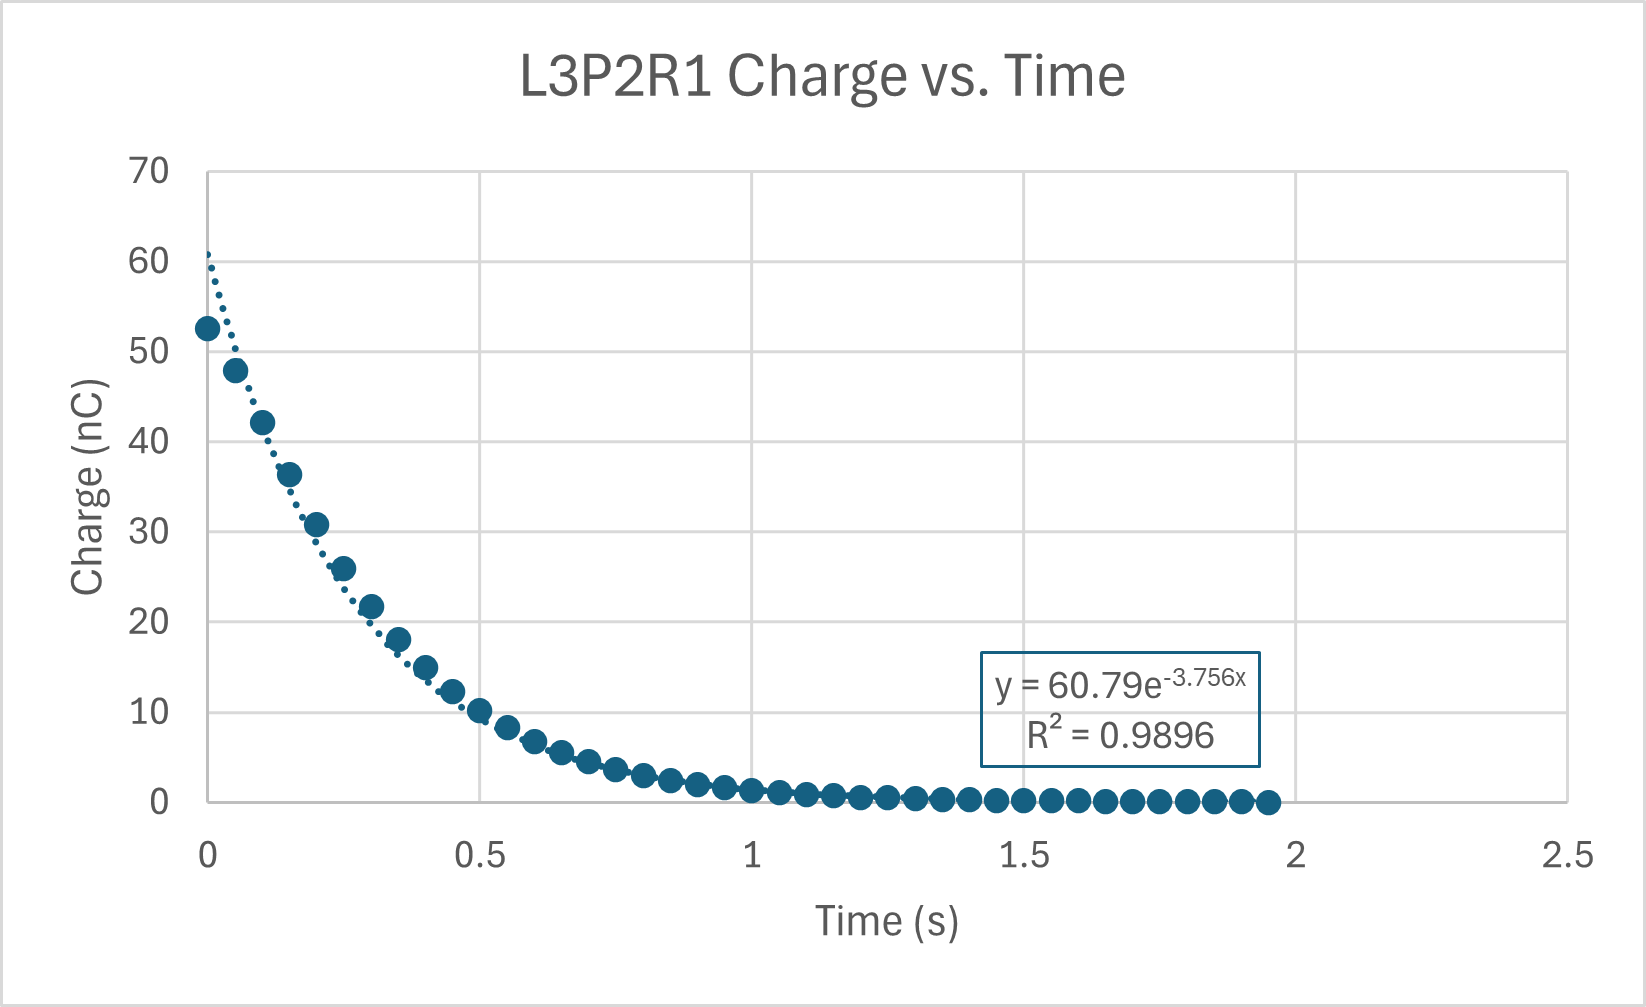
\includegraphics[width=0.8\linewidth]{../figures/L3P2R1_QvT.png}\\
    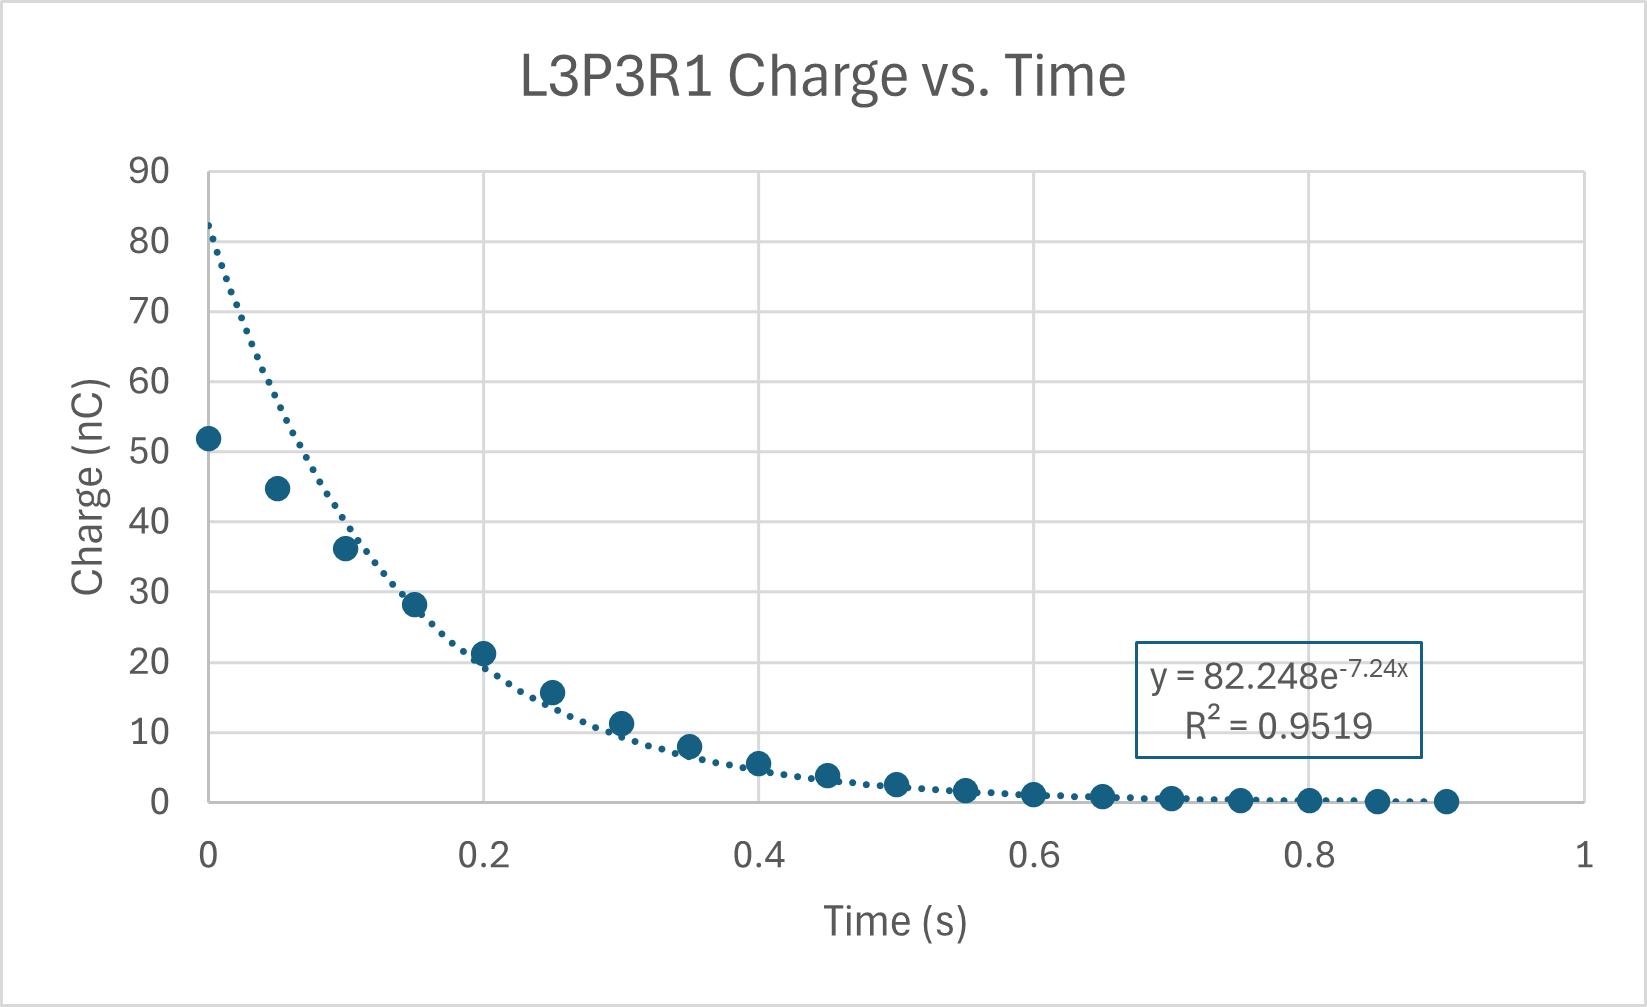
\includegraphics[width=0.8\linewidth]{../figures/L3P3R1_QvT.png}
    \caption{Charge vs.\ time during discharge for both capacitors. The exponential fit shows strong agreement with theoretical decay.}
    \label{fig:QvT}
\end{figure}

\begin{figure}[H]
    \centering
    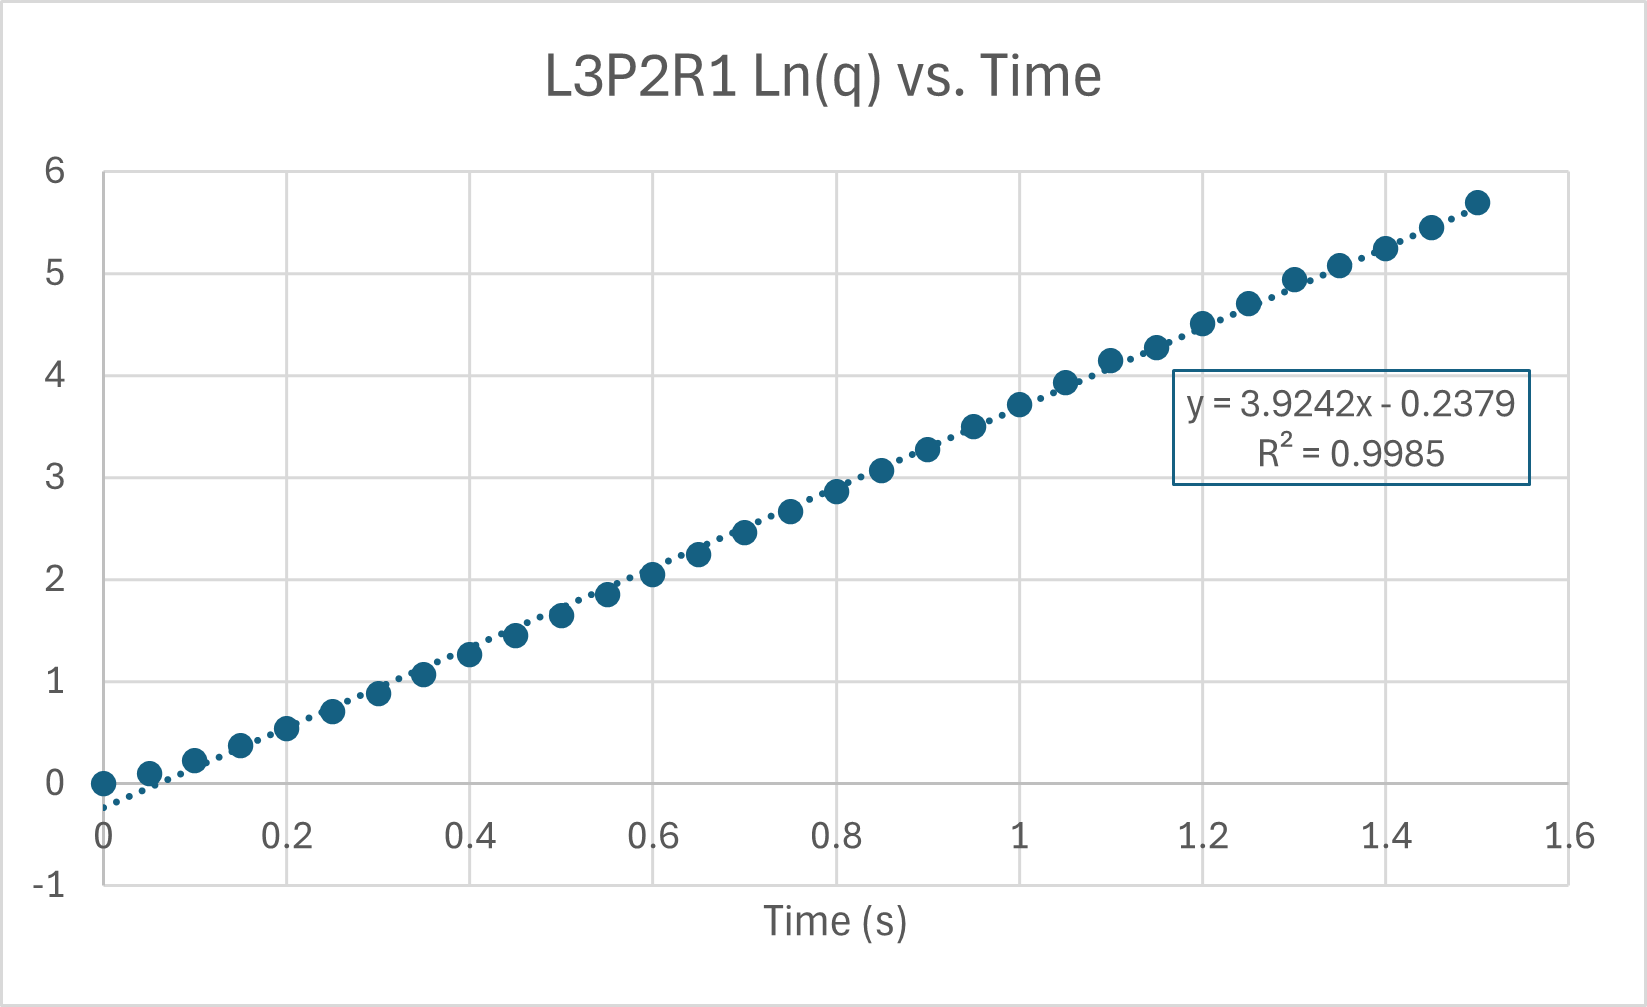
\includegraphics[width=0.8\linewidth]{../figures/L3P2R1_ln(Q)vT.png}\\
    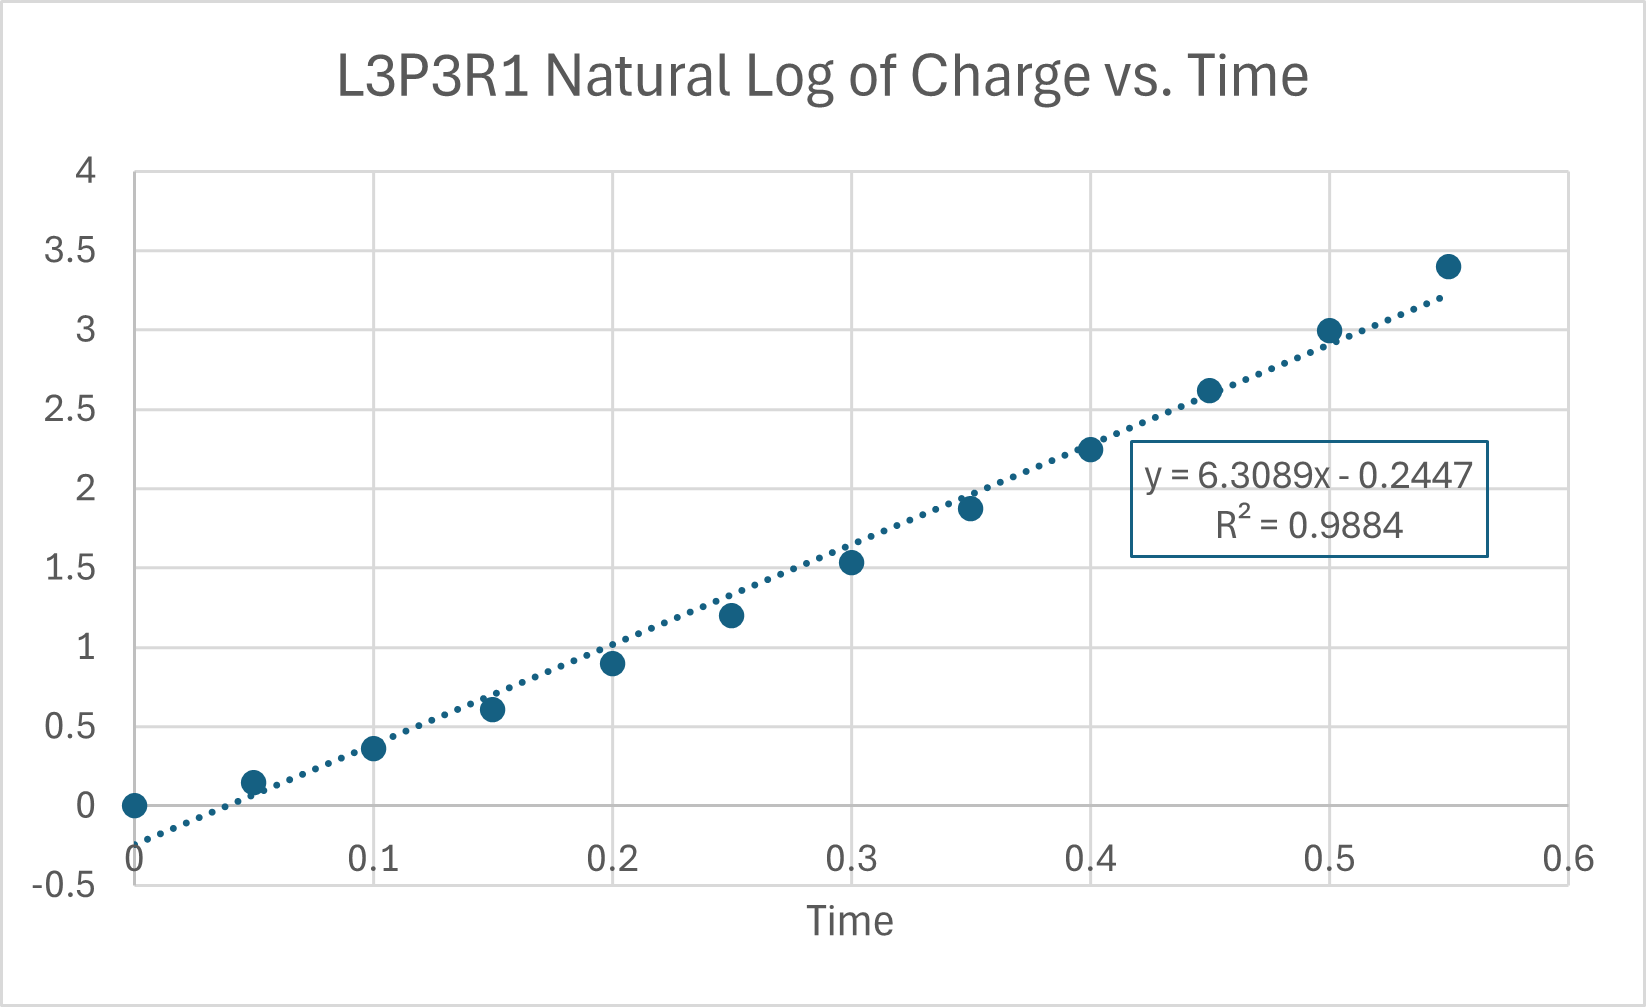
\includegraphics[width=0.8\linewidth]{../figures/L3P3R1_ln(Q)vT.png}
    \caption{Natural logarithm of charge ratio vs.\ time during discharge for both capacitors. The linear fit confirms the exponential decay model.}
    \label{fig:ln(Q)vT}
\end{figure}

\begin{figure}[H]
    \centering
    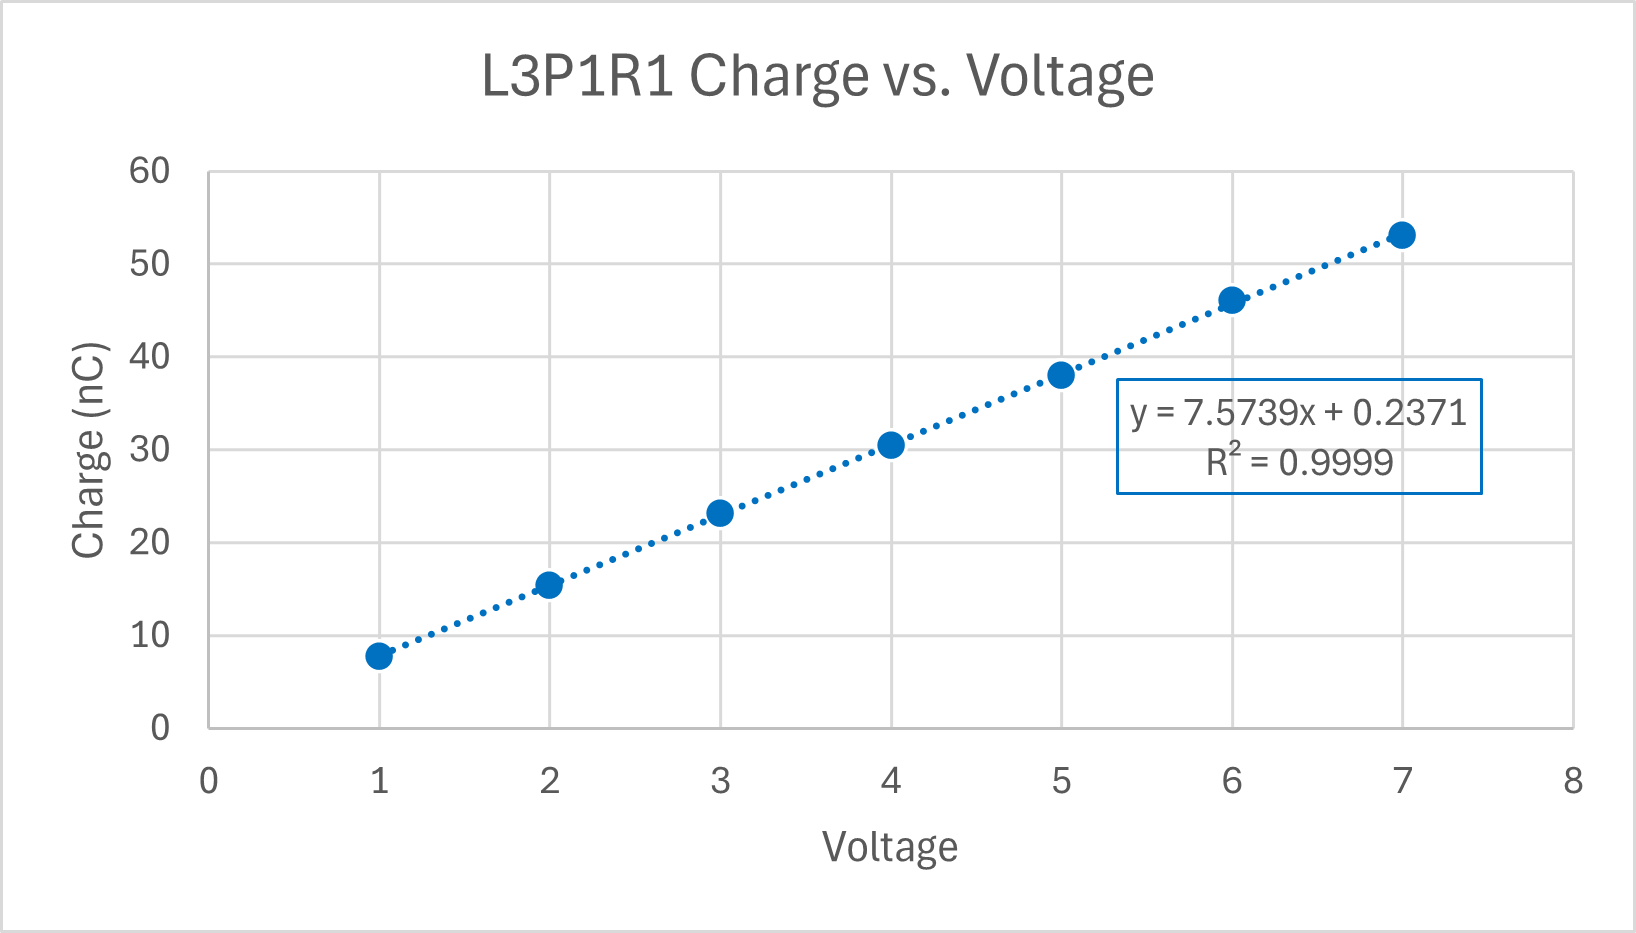
\includegraphics[width=0.8\linewidth]{../figures/L3P1R1_QvV.png}
    \caption{Charge vs.\ voltage for the \SI{0.01}{\micro\farad} charge sensor. The linear fit indicates a capacitance of \SI{0.0075739}{\micro\farad}.}
    \label{fig:QvV}
\end{figure}

\section{Error Analysis}
Overall, experimental results were consistent with theoretical expectations.
Small deviations were likely due to:
\begin{itemize}
    \item Resistance in the power supply and wiring, slightly altering $R$
    \item Sensor calibration drift leading to error in charge readings
    \item Voltage fluctuations during switching between charge and discharge
    \item Manual timing differences when identifying the discharge portion in LoggerPro
\end{itemize}
The linear fits of $\ln(Q/Q_0)$ vs.\ $t$ produced $R^2$ values near 0.9985 and 0.9884 respectively, indicating a strong exponential relationship.

Future improvements could include automated switching, longer data collection durations, and averaging multiple runs to reduce random error.

\section{Conclusion}
The experiment successfully demonstrated the theoretical relationships between charge, voltage, and capacitance in capacitors
The experiment also confirmed the exponential decay behavior in RC discharge circuits.
The calculated capacitance values were within 11\% and 45\% respectively of accepted values for both capacitors, corroborating the validity of the experiment.
The time constants obtained were consistent with $\tau = RC$, and the results strongly support the exponential discharge model.
Likely sources of error primarily arose from measurement timing and minor sensor inaccuracies.
Overall, the data supported the theoretical model for both the charge–voltage and discharge–time relationships.

\appendix
\section{Full Data Files}
\noindent The original data file is attached here: \attachfile{..\data\raw\Physics-II_Lab-3.xlsx}

\end{document}
